\chapter{Implementation Details}
\section{Project structure}
We decided to put every algorithm of the specification in its own file together with related unit tests. The files are structured according to the actors of the protocol, for example:

\begin{itemize}
	\item \textbf{Common}: contains common cryptopgraphic algorithms and the security parameters used by multiple algorithms
	\item \textbf{ElectionAuthority}: contains all the algorithms used by the election authority
	\item \textbf{PrintingAuthority}: contains all the algorithms used by the printing authority
	\item \textbf{VotingClient}: contains all the algorithms used by the voting client
	\item \textbf{ElectionAdministration}: contains all the algorithms used by the election administrator
	\item \textbf{Utils}: contains helper classes and miscellaneous utility functions
	\item \textbf{Protocol}: contains the protocol implementation
	\item \textbf{profiles}: contains JSON files that are used to define election parameters
\end{itemize}

\section{Public parameters}
There exist two types of public parameters:

The \textbf{security relevant parameters}, e.g:

\begin{itemize}
	\item The order of the prime groups: $p$, $\prime{p}$, $\hat{p}$
	\item The length of the voting, confirmation, return and finalization codes
	\item The number of authorities: $s$
\end{itemize}

and \textbf{public election parameters}, e.g.:

\begin{itemize}
	\item The size of the electorate: $N_E$
	\item The number of candidates: $n$
	\item The list of candidate descriptions: $c$
\end{itemize}

The security parameters are typically used within the algorithms and remain unchanged for a longer time period, whereas the public election parameters are only used by the protocol implementations and change with every election.

The object \texttt{SecurityParams} holds all security relevant parameters and is injected as an additional function argument to all algorithms. Several different \texttt{SecurityParams} objects are created initially, which contain all the parameters according to the recommendations in the CHVote specification document ("level 0" for testing purposes and "level 1" through "level 3" for actual use of the protocol). This approach allows us to use different levels of security during development of the algorithms and protocols. For simple unit testing we used "level 0" in order to inject the security parameters recommended for testing puposes. For actual test runs of the project the security parameters from "level 2" were used.

The public election parameters are defined in a JSON file and simply read as an object which is directly accessed by the protocol. If an algorithm needs to know certain election parameters (like the size of the electorate $N_E$), these values are typically derived from vectors that they have access to, so they do not require specific knowledge of these parameters.

The following is a exmaple for the contents of a JSON file containing all the parameters:

\begin{minted}[linenos,tabsize=2,breaklines]{json}
{
  "autoGenerateVoters" : true,
  "numberOfVotersToGenerate" : 50,
  "voters" : [
    {
      "name" : "Voter1",
      "selection" : "1,5"
    },
    {
      "name" : "Voter2",
      "selection" : "0,5"
    },
    {
      "name": "Voter3",
      "selection": "0,5"
    }
  ],
  "t" : 2,
  "n" : [5, 3],
  "c" : ["Hillary Clinton", "Donald Trump", "Vladimir Putin", "Marine Le Pen", "May", "Yes", "No", "Empty"],
  "k" : [1, 1],
  "E" : [[1, 1], [1, 1], [1, 1]],
  "securityLevel" : 2,
  "deterministicRandomGeneration" : false
}
\end{minted}

\section{Coding style}
The following source code sample shows a typical implemation of an algorithm (in this exmaple, algorithm 7.18 according to the CHVote specification).

\begin{minted}[linenos,tabsize=2,breaklines]{python}
import unittest
import os, sys
from gmpy2 import mpz
import gmpy2

sys.path.append(os.path.dirname(os.path.dirname(os.path.abspath(__file__))))

from Utils.Utils                    import AssertMpz, AssertList, AssertClass, AssertString
from Crypto.SecurityParams          import SecurityParams, secparams_l0
from Utils.ToInteger                import ToInteger
from VotingClient.GetSelectedPrimes import GetSelectedPrimes
from VotingClient.GenQuery          import GenQuery
from VotingClient.GenBallotProof    import GenBallotProof
from UnitTestParams                 import unittestparams
from Types                          import Ballot
from Utils.StringToInteger          import StringToInteger

def GenBallot(X_bold, s, pk, secparams):
    """
    Algorithm 7.18: Generates a ballot based on the selection s and the voting code X. The
    ballot includes an OT query a and a proof pi. The algorithm also returns the random
    values used to generate the OT query. These random values are required in Alg. 7.27
    to derive the transferred messages from the OT response, which itself is generated by Alg. 7.25.

    Args:
        X_bold (str):                       Voting Code X ∈ A_X^l_X
        s (list of int):                    Selection s = (s_1, ... , s_k), 1 <= s_1 < ... < s_k
        pk (mpz):                           ElGamal key pk ∈ G_p \ {1}
        secparams (SecurityParams):         Collection of public security parameters

    Returns:
        tuple:                              alpha = (r, Ballot) = (r, (x_hat, a, b, pi))
    """

    AssertMpz(pk)
    AssertList(s)
    AssertClass(secparams, SecurityParams)

    x = mpz(StringToInteger(X_bold, secparams.A_X))
    x_hat = gmpy2.powmod(secparams.g_hat, x, secparams.p_hat)

    q_bold = GetSelectedPrimes(s, secparams)                    # q = (q_1, ... , q_k)
    m = mpz(1)

    for i in range(len(q_bold)):
        m = m * q_bold[i]

    if m >= secparams.p:
        return None

    (a_bold, r_bold) = GenQuery(q_bold, pk, secparams)
    a = mpz(1)
    r = mpz(0)

    for i in range(len(a_bold)):
        a = (a * a_bold[i]) % secparams.p
        r = (r + r_bold[i]) % secparams.q

    b = gmpy2.powmod(secparams.g,r, secparams.p)
    pi = GenBallotProof(x,m,r,x_hat,a,b,pk, secparams)
    alpha = Ballot(x_hat,a_bold,b,pi)

    return (alpha, r_bold)

class GenBallotTest(unittest.TestCase):
    def testGenBallot(self):
        selection = [1,4]       # select candidates with indices 1,4
        (ballot, r) = GenBallot(unittestparams.X, selection, unittestparams.pk, secparams_l0)
        print(ballot)
        print(r)

if __name__ == '__main__':
    unittest.main()
\end{minted}

All algorithms contain a short description, which was taken as-is from the specification document, as well as a comment (Google-style documentation string), which can be used to automatically generate code documentation. The algorithm itself is implemented as close to the specification as possible, using the same variable names and (as far as the language supports it) similar control structures:

\begin{itemize}
	\item The suffix \texttt{\_bold} for emphasized (bold) variables, e.g. \texttt{p\_bold} for \textbf{p}
	\item The suffix \texttt{\_hat} for variables with a hat, e.g. \texttt{a\_hat} for $\hat{a}$
	\item The suffix \texttt{\_prime} for variables with a prime, e.g. \texttt{a\_prime} for $a'$
	\item etc.
\end{itemize}

Each file also contains unit test relevant to the specific algorithm (if unit testing was considered useful for the particular algorithm).

The following example shows the similarities between the algorithm pseudo code and the actual implmentation in Python:

\begin{multicols}{2}
%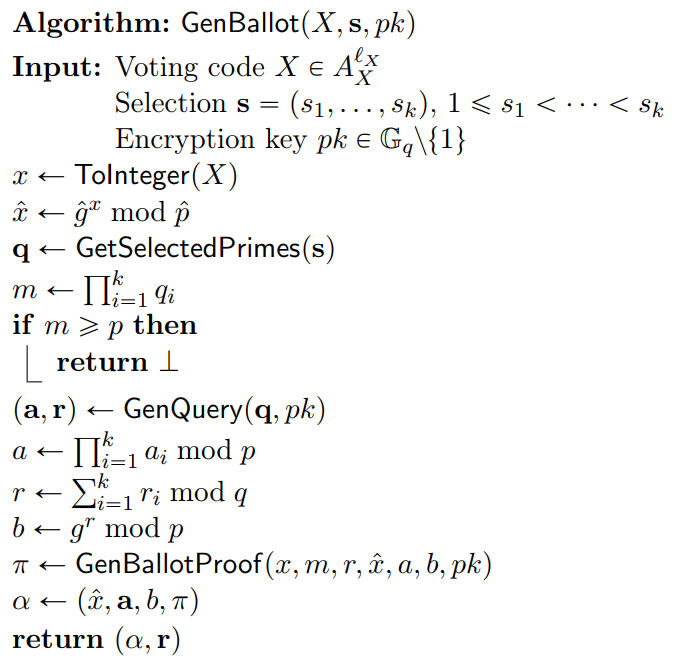
\includegraphics[width=0.46\textwidth]{images/genballot.png}
\columnbreak
\begin{minted}[fontsize=\scriptsize]{python}
x = mpz(StringToInteger(X_bold, secparams.A_X))
x_hat = gmpy2.powmod(secparams.g_hat, x, secparams.p_hat)
q_bold = GetSelectedPrimes(s, secparams)

m = mpz(1)
for i in range(len(q_bold)):
    m = m * q_bold[i]

if m >= secparams.p:
    return None

(a_bold, r_bold) = GenQuery(q_bold, pk, secparams)
a = mpz(1)
r = mpz(0)

for i in range(len(a_bold)):
    a = (a * a_bold[i]) % secparams.p
    r = (r + r_bold[i]) % secparams.q

b = gmpy2.powmod(secparams.g,r, secparams.p)
pi = GenBallotProof(x,m,r,x_hat,a,b,pk, secparams)
alpha = Ballot(x_hat,a_bold,b,pi)

return (alpha, r_bold)
\end{minted}
\end{multicols}

\subsection{Return types}
In most cases, when an algorithm returns more than a scalar datatype, tuples are used. Tuples allow to return multiple values from a function:

\begin{minted}[linenos,tabsize=2,breaklines]{python}
def foo():
   return (1, 2)

def main():
   a, b = foo()
\end{minted}

This way a lot of the source code looked very similar to the pseudo code in the CHVote specification. For more complex data types or return values that are used more often, named tuples were used. The data type "namedtuple" is like a lightweight class and allows access to named properties.

\begin{minted}[linenos,tabsize=2,breaklines]{python}
Ballot = namedtuple("Ballot", "x_hat, a_bold, b, pi")

def main():
   Ballot b = getBallot()
   x_hat = b.x_hat
\end{minted}

By following this approach we can avoid having hundreds of classes only used to pass data structures between the algorithms.

\section{Protocol}
Upon completion of the algorithm implmentation we have built a protocol layer according to the specification. For that purpose we created a seperate entity for every protocol participant, namely the following ones:

\begin{itemize}
	\item \textbf{VotingClient}
	\item \textbf{ElectionAuthority}
	\item \textbf{BulletinBoard}
	\item \textbf{PrintingAuthority}
\end{itemize}

The following example shows the first step of protocol 6.5:

\begin{minted}[linenos,tabsize=2,breaklines]{python}
def castVote(self, s, autoInput, secparams):
		self.pk = GetPublicKey(self.bulletinBoard.pk_bold,secparams)

		X = input('Enter your voting code: ')
		(self.alpha, self.r) = GenBallot(X, s, self.pk, secparams)

		return (self.alpha, self.r)
\end{minted}

Finally, within a \textbf{VoteSimulation}, all these entities are instantiated and perform their protocol steps in order. The following example illustrates the vote casting phase:

\begin{minted}[linenos,tabsize=2,breaklines]{python}
votingClients = [VotingClient(i, self.voters[i], self.rawSheetData[i], self.bulletinBoard) for i in range(len(self.voters))]
for votingClient in votingClients:
		# Get selection (protocol 6.4)
		s = votingClient.candidateSelection(autoInput, self.secparams)

		# Generate ballot & send oblivious transfer query (protocol 6.5)
		(ballot, r) = votingClient.castVote(s, autoInput, self.secparams)

		# Generate oblivious transfer response & check ballot (protocol 6.5)
		responses = [(authority.name, authority.runCheckBallot(votingClient.i, ballot, self.secparams)) for authority in self.authorities]
		for res in responses: print("Ballot validity checked by authority %s: %r" % (res[0], res[1]))
\end{minted}
